%!TEX root = ./ERL Industrial Robots-rulebook.tex

%--------------------------------------------------------------------
%--------------------------------------------------------------------
\subsection{Environment Structure and Properties}
\label{ssec:StructureProperties}

\noindent
The following set of scenario specifications must be met by the \erlir environment.
%-----------
\begin{envSpec}[Structured Environment]
The environment can consists of various numbers of spatial areas:
	\begin{enumerate}
	\renewcommand{\itemsep}{0.1ex}
	\item rows of shelves
	\item rows of workstations
	\end{enumerate}
	Figure \ref{fig:ArenaArea} shows an example of these areas in the \erlir environment.
The spatial areas extend beyond the space occupied by the respective workstations or objects and include the surrounding area as well. 
\end{envSpec}

%-----------
\begin{envSpec}[Flat Environment]
	All spatial areas are located on the same level, except where 
	specified otherwise. There are no stairs in the environment.
\end{envSpec}

%-----------
\begin{envSpec}[Spatial Areas and Rooms]
The factory is a single, large open space; there are no rooms separated by walls in the environment. 
Spatial areas can be partially separated by dividing or protective walls or other objects present in the factory (e.g. shelves, workstations, platforms, tables).
\end{envSpec}

%-----------

\begin{figure}[!htbp]
  \begin{center}
  	  \scalebox{1.0}[1.0]{%
  		  \includegraphics[width=140mm,angle=0, trim=0px 0px 0px 0px,clip]%
	  		{./fig/WorkArenaBRSUSpatialArea.jpg}%
			}%
	   	\caption{Example of the spatial areas in the \erlir environment. The spatial areas are shelves (red), force fitting workstation (blue), conveyor belt (green), drilling workstation (orange) and assembly workstation (yellow).}
  	\label{fig:ArenaArea} 
  \end{center}
\end{figure}

%-----------
\begin{envSpec}[Dimensions]
	\label{scenspec:dimensions}
	The precise dimensions and the arrangement of the spatial areas are not predefined, but estimated sizes are given. 
	The estimated sizes of the spatial areas are as follows: workstations $2m\times2m $ and shelves $5m\times0,5m$.
	The bounding box of the environment has a minimum area of $16 m^2$ and a maximum area of $100 m^2$. More space is used, when areas and workstations are doubled for teams working in parallel.
\end{envSpec}

%-----------
\begin{envSpec}[Set of Shelves]
The shelves-area is a set of connected shelves and each shelves has two level (upper level and lower level).
The robot can take and/or deliver objects from the shelves (through the containers or directly onto shelves).
Figure \ref{fig:ArenaArea} shows an example of the shelves-area made from two set of shelves.
\end{envSpec}

%-----------
%\begin{envSpec}[Force Fitting Workstation]
%Force fitting workstation has a table for temporarily storing handled parts. 
%The table is part of the force fitting machine which is operated by a robot or human worker. 
%On one side is the assembly aid tray rack to attach filled or unfilled aid trays.
%\end{envSpec}

%-----------
%\begin{envSpec}[Drilling Workstation]
%Drilling workstation consists of a storing area to store ``file card'' boxes and the drilling machine. 
%\end{envSpec}

%-----------
%\begin{envSpec}[Conveyor Belt]
%	The conveyor belt transports parts from outside of the arena into the area.
%	%At the end of the conveyor belt, parts fall down on an exit ramp in a predefined position through guiders where they can be taken by the robot.
%\end{envSpec}

%-----------
\begin{envSpec}[Workstations]
Workstations are used as storage areas for objects. They may be accessible from different locations, i.e. it might be possible to reach a workstation from two or more sides. Additional, there are workstations of different heights present in the environment, ranging from 0 cm up to 15 cm. If a workstation has a height of 0 cm, a tape will mark the area (see Figure \ref{fig:barrier_tape_0cm}). The tape will be taped on the floor and is blue/white striped. This tape may be crossed by the robot and does not count as a collision.
\end{envSpec}

\begin{figure} [h!]
	\begin{center}
		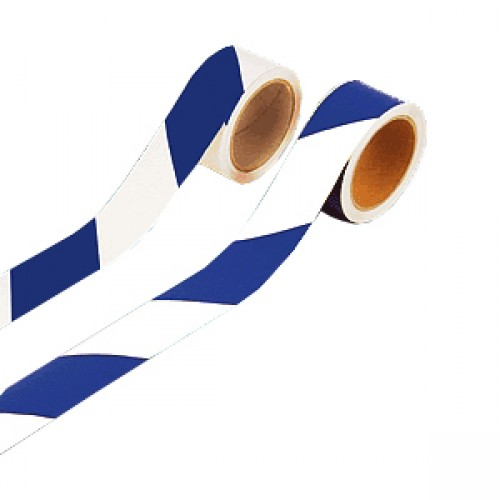
\includegraphics[height = 2.5cm]{pics/atwork/barrier_tape/barrier_tape_0cm_area.jpg}
	\end{center}
	\caption{Barrier tape used to mark workstations with 0 cm height.}
	\label{fig:barrier_tape_0cm}
\end{figure}

%-----------
%\begin{envSpec}[Rotating Table]
%	The rotating table can, similar to a usual workstation, store any kind of object. But compared to a workstation the rotating table is not static and rotating at a constant speed.
%
%\end{envSpec}
	
\begin{envSpec}[Barrier Tape as Virtual Walls]
The environment may include virtual walls marked by either striped yellow/black or white/red barrier tape on the floor (see Figure \ref{fig:barrier_tape}). If any part of a robot passes over such a tape it is considered as a collision with a obstacle. The red/white tape is used to frame the entrance and exit area. The robot is allowed to cross this kind of barrier only at the beginning of a test to enter arena and at the end for leaving. In contrast, the yellow/black one denotes an obstacle which the robot is never allowed to cross.
\end{envSpec}

\begin{figure} [h!]
	\centering
	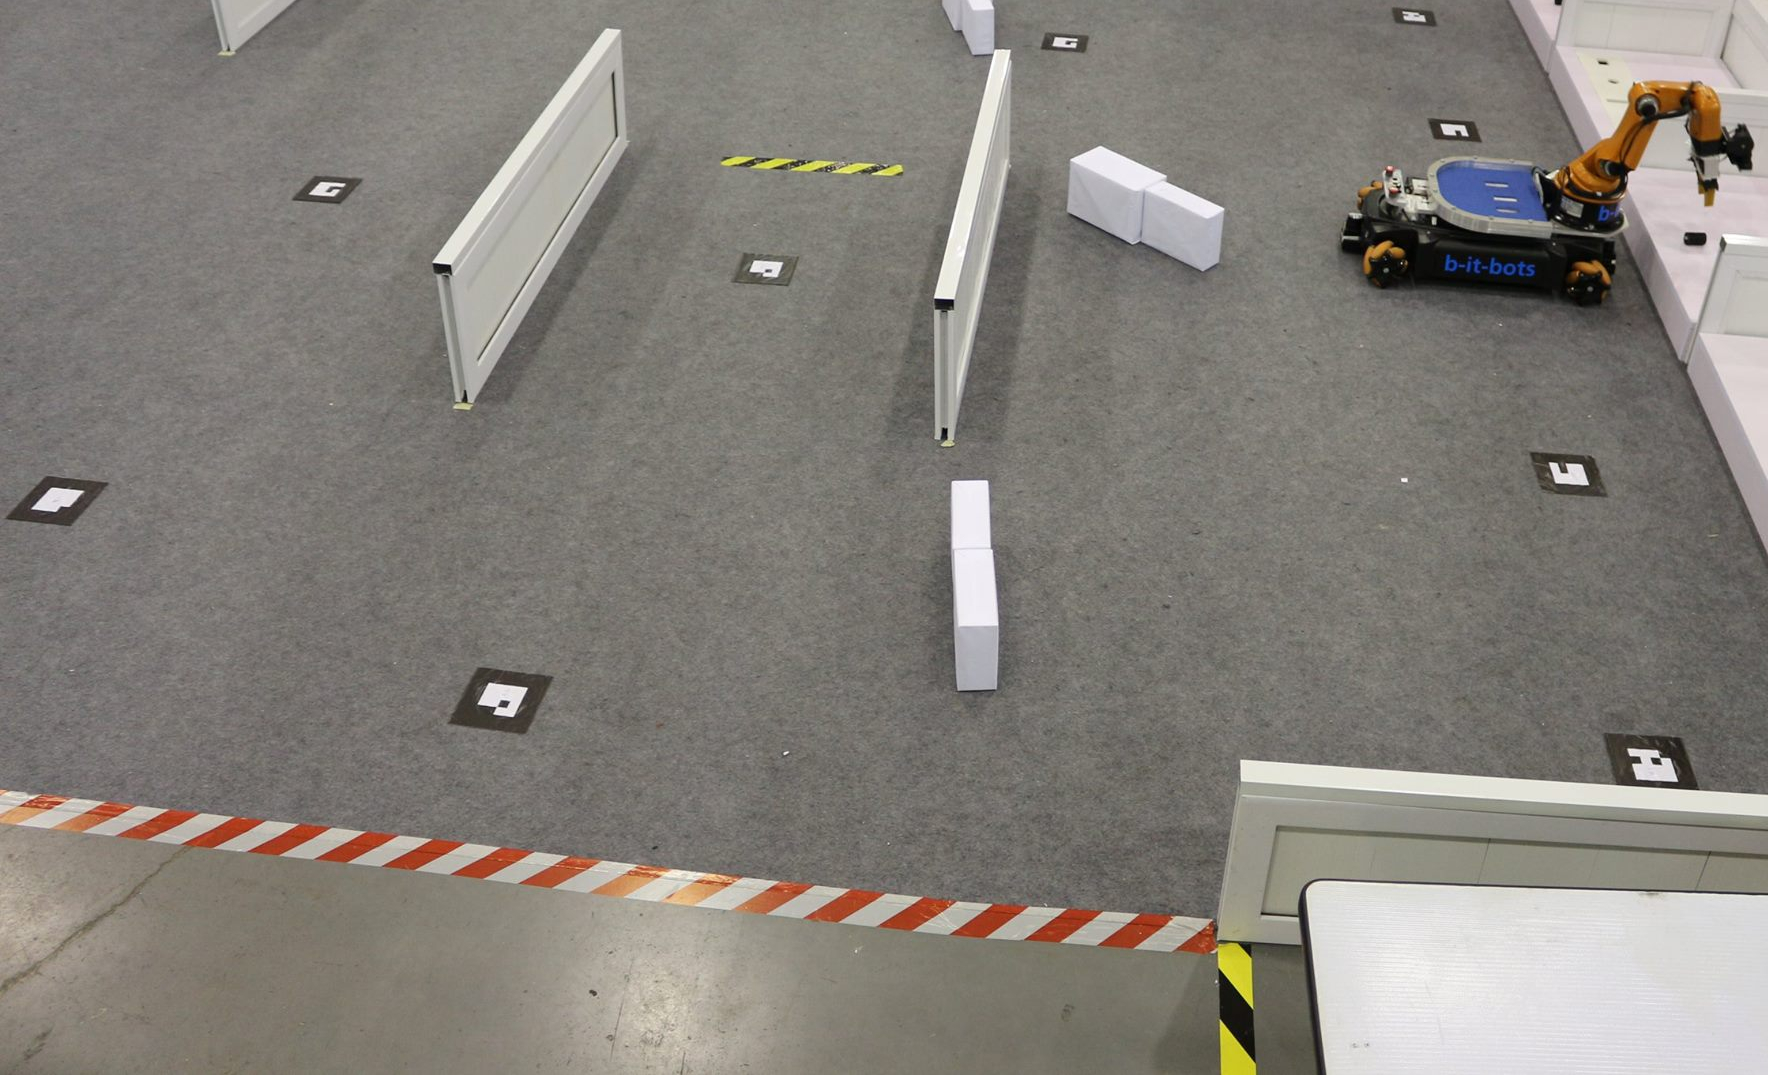
\includegraphics[width= 0.7\textwidth ]{pics/atwork/barrier_tape/barrier_tapes_in_china15.jpg}
	\caption{Example of the different kind of barrier tapes. The red/white tape is used for the entrance and exit, while the yellow/black one denotes an obstacle.}
	\label{fig:barrier_tape}
\end{figure}

%
%
%--------------------------------------------------------------------
% EOF
%--------------------------------------------------------------------
